%-----------------------------------------------------------------------------------------------------------------
%% Section 1
\chapter{Question 1: Mass Actuator System}
\label{chap:q1}

The natural frequency $\omega_n$ of the mass actuator system in Figure~\ref{fig:q1} \cite{assign} below is of interest.

\begin{figure}[H]
	\centering
	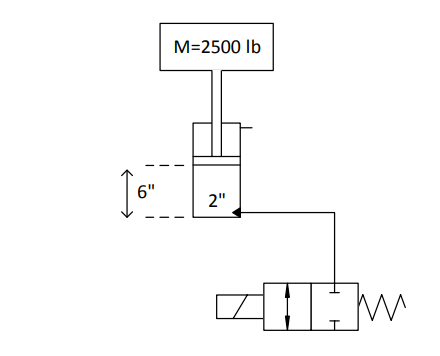
\includegraphics[scale=0.75]{q1}
	\caption{Question 1 circuit schematic.}
	\label{fig:q1}
\end{figure}

Constant parameters are listed in Table~\ref{tab:q1_param}. Furthermore, the following assumptions are made \cite{assign}.
\begin{itemize}
\item De-energized directional valve
\item Rigid cylinder walls
\item No air content
\end{itemize}

\begin{table}[H]
  \centering
  \caption{Given parameters.}
    \begin{tabular}{cccc}
    \toprule
    \textbf{Description} & \textbf{Symbol} & \textbf{Value } & \textbf{Unit} \\
    \midrule
    Mass  & $m$   & 2500  & lbm \\
    Stroke & $l$   & 6     & in \\
    Diameter & $D$   & 2     & in \\
    Bulk modulus & $\beta$ & 260000 & psi \\
    \bottomrule    
    \end{tabular}
  \label{tab:q1_param}
\end{table}

To find $\omega_n$, the system's dynamics must be derived. This is done with the hydraulic system's equivalent mass spring damper model. Applying Newton's second law to the free body diagram in Figure~\ref{fig:q1_fbd} will yield the final result in \ref{eq:q1_newt}.

\begin{figure}[H]
	\centering
	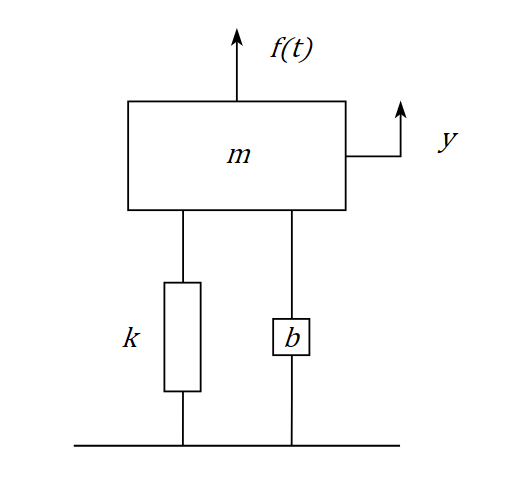
\includegraphics[scale=0.75]{q1_fbd}
	\caption{Free body diagram.}
	\label{fig:q1_fbd}
\end{figure}

\begin{equation}
	\label{eq:q1_newt}
	m \ddot{y} = f(t) - b\dot{y} - k y
\end{equation}

Taking the Laplace of \ref{eq:q1_newt} with zero initial conditions and rearranging to get in standard plant model form \ref{eq:q1_tfactual}.

\begin{equation*}
	ms^2 Y(s) + b s Y(s) + k Y(s) = F(s)
\end{equation*}

\begin{equation}
	\label{eq:q1_tfactual}
	P(s) = \frac{Y(s)}{F(s)} = \frac{\frac{1}{m}}{s^2 + \frac{b}{m}s + \frac{k}{m}}
\end{equation}

From this, the natural frequency can be extrapolated from the ideal second order transfer function $P(s)$ \ref{eq:q1_tfideal}.
\begin{equation}
	\label{eq:q1_tfideal}
	P(s)= \frac{\omega_n^2}{s^2+2\zeta\omega_n s + \omega_n^2}
\end{equation}

Comparing like coefficients yields a final expression for $\omega_n$ \ref{eq:q1_wn}.
\begin{equation}
	\label{eq:q1_wn}	
	\omega_n = \sqrt{\frac{k}{m}}	
\end{equation}

The mass $m$ is given in Table~\ref , therefore it is required to find the equivalent stiffness constant $k$. This is done with the bulk modulus equation $\beta$ \ref{eq:q1_beta}.
\begin{equation}
	\label{eq:q1_beta}
	\beta = - \frac{\Delta p V_0}{\Delta V}	
\end{equation}

Realizing that $V_0 = AL$ and $\Delta V = Ax$, rearranging \ref{eq:q1_beta} for $\Delta p$ and comparing with well known $p =F/A$ relation yields \ref{eq:q1_f}.

\begin{equation}
	\label{eq:q1_f}
	\Delta p = \beta \ \frac{y}{l} = \frac{F}{A} \Rightarrow F = \frac{A\beta}{l}y 	
\end{equation}

Knowing that $F = ky$, comparing the result of \ref{eq:q1_f} yields the final relation for the equivalent stiffness $k$ in [lbf/in]. 

\begin{equation}
	\label{eq:q1_k}
	 k = \frac{A\beta}{l} 	
\end{equation}

Note that the above units of $k$ are equivalent to [lbm/$\Unit{s^2}$] hence, \ref{eq:q1_wn} yields a frequency in [rad/s].\\

Applying the above equations with parameters from \cite{assign} yields the final results in Table~\ref{tab:q1_ans}.
 
\begin{table}[H]
  \centering
  \caption{Calculated values.}
    \begin{tabular}{cccc}
    \toprule    
    \textbf{Description} & \textbf{Symbol} & \textbf{Value } & \textbf{Unit} \\
    \midrule
    Area  & $A$   & 3.142 & $\Unit{in^2}$ \\
    Volume & $\forall_0$ & 18.850 & $\Unit{in^3}$ \\
    Stiffness & $k$   & 1.361E+05 & lbf/in \\
    Natural frequency & $\omega_n$ & 7.379 & rad/s\\
	\bottomrule    
    \end{tabular}
  \label{tab:q1_ans}
\end{table}

The natural frequency of the system is \textbf{7.379 [rad/s]} or \textbf{1.174 [Hz]}.

%-----------------------------------------------------------------------------------------------------------------
%% Section 2
\chapter{Accumulator}
\label{chap:q2}

The following circuit schemic in Figure~\ref{fig:q2} below is given \cite{assign}.

\begin{figure}[H]
	\centering
	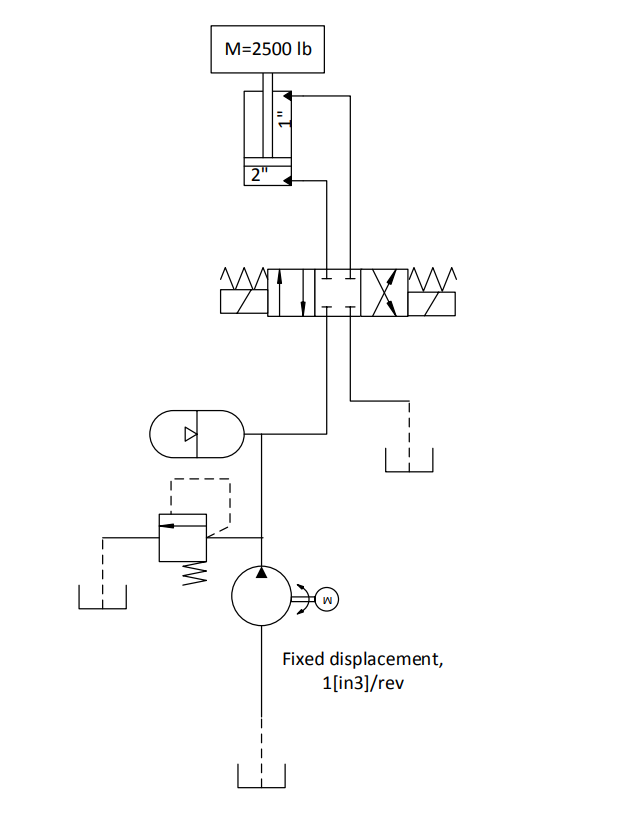
\includegraphics[scale=0.75]{q2}
	\caption{Question 2 circuit schematic.}
	\label{fig:q2}
\end{figure}

Constant parameters are listed in Table~\ref{tab:q2_param}. 
\begin{table}[H]
  \centering
  \caption{Question 2 constant parameters.}
    \begin{tabular}{cccc}
    \toprule
    \textbf{Description} & \textbf{Symbol} & \textbf{Value } & \textbf{Unit} \\
    \midrule
    Piston diameter & $D_P$ & 2     & in \\
    Rod diameter & $D_R$ & 1     & in \\
    Stroke length & $L$   & 10    & in \\
    Mass  & $m$   & 2500  & lbm \\
    Actuator speed & $v$   & 45    & in/s \\
    Relief valve opening pressure & $p_{RV}$ & 230   & bar \\
    Accumulator pre-charge pressure & $p_A$ & 1800  & psig \\
    Pump speed & $N$   & 1700  & RPM \\
    Pump displacement volume & $V_P$ & 1     & $\Unit{in^3/rev}$ \\
    Pump volumetric efficiency & $\eta_V$ & 100     & \% \\
    \bottomrule    
    \end{tabular}
  \label{tab:q2_param}%
\end{table}%


Assumptions:
\begin{itemize}
\item Actuator initially fully retracted
\item Positive displacement pump
\item Return line pressure is 0 psig $\Rightarrow$ 14.7 psi
\item Accumulator air is an ideal gas
\item Accumulator effective volume when no oil in it
\end{itemize}

\section{Hydraulic Pump Pressure}

The required hydraulic pressure at the pump outlet $p_p$ is desired. To find this value, it is first required to find the pressure exerted on the piston $p_1$. Knowing that $p=F/A$ and that the force due the the mass is $W= F_{\Unit{lbf}}=32.174\cdot m_{\Unit{lbm}}$, this value is calculated with \ref{eq:q2_p1}.

\begin{equation}
	\label{eq:q2_p1}
	 p_1 = \frac{W}{A_1} + p_{ATM}
\end{equation}

Flow rate $Q_1$ into cylinder is \ref{eq:q2_q1}. 

\begin{equation}
	\label{eq:q2_q1}
	 Q_1 = A_1 v
\end{equation}

Pressure loss $\Delta p$ across the valve for each land is defined as \ref{eq:q2_ploss}.

\begin{equation}
	\label{eq:q2_ploss}
	 \Delta p = 725 \left( \frac{Q_1}{100} \right)^2
\end{equation}

Note that the above equation is for $p$ in psi and $Q$ in $\Unit{in^3/s}$ for consistency in units. A factor of 14.5 is added from the original equation in \cite{assign} since $p_{\Unit{bar}} = 14.5 \cdot p_{\Unit{psi}}$.\\

Finally, sthe pump pressure $p_P$ is simply the required piston pressure plus the loses, \ref{eq:q2_ppump}.
\begin{equation}
	\label{eq:q2_ppump}
	 p_p = p_1 + 2\Delta p
\end{equation}

Results in Table~\ref{tab:q2a_ans}.

\begin{table}[H]
  \centering
  \caption{Question 2, part A results.}
    \begin{tabular}{cccc}
    \toprule
    \textbf{Description} & \textbf{Symbol} & \textbf{Value } & \textbf{Unit} \\
    \midrule
    Pound force & $W$   & 80435 & lbf \\
    Pisten end area & $A_1$ & 3.142 & $\Unit{in^2}$ \\
    Piston end pressure & $p_1$ & 25618 & psi \\
    Required piston flow rate & $Q_1$ & 141.37 & $\Unit{in^3/s}$ \\
    Pressure loss per valve land & $\Delta p$ & 1449  & psi \\
    Pump pressure & $p_P$ & X & psi \\
    \bottomrule
    \end{tabular}
  \label{tab:q2a_ans}
\end{table}%

Hence in can be concluded that a pump pressure of \textbf{X psi} or \textbf{X bar} is required.

%%% Archive
%
%Recall that $\eta_V = Q_A/Q_T \therefore Q_T = Q_A \because \eta_V = 1$. From this the actual pump flow rate is calculated as 
%
%
%\begin{equation}
%	\label{eq:q2_qa}
%	 Q_A = \frac{1}{60} V_D N
%\end{equation}
%
%A factor of 1/60 is added for $\Unit{in^3/min} \rightarrow \Unit{in^3/s}$.
% Since $p_{\Unit{psig}}= p_{\Unit{psi}} - 14.7$ and $p_{\Unit{bar}} = 14.5 \cdot p_{\Unit{psi}}$ .


\section{Accumulator Effective Volume}

Assuming that the accumulator is isothermal, the accumulator's effect gas volume $V_1$ is calculated with \ref{eq:q2_acum}.

\begin{equation}
	\label{eq:q2_acum}
	V_1 = \frac{\Delta V}{\frac{p_1}{p_2}-\frac{p_1}{p_3}}
\end{equation}

Where $p_1 \equiv$ accumulator's pre charged pressure (or $p_a$ see Table \ref{tab:q2_param}), $p_2 \equiv$ pump pressure (or $p_P$ see Table \ref{tab:q2a_ans}) and $p_3 \equiv$ maximum pressure (or $p_RV$ see Table \ref{tab:q2_param}).\\

With \ref{eq:q2_acum}, the accumulator's effective gas volume is calculated as \textbf{X [in\textsuperscript{3}]}.

%-----------------------------------------------------------------------------------------------------------------
%% Section 3
\chapter{Cascade Design}
\label{chap:q3}

It is desired to design a pneumatic cascade circuit for the sequence in \ref{eq:q3_cd} \cite{assign}.

\begin{equation}
	\label{eq:q3_cd}
	 A^+ B^+ B^- A^- C^+ C^- D^+ D^- 	
\end{equation}

The sequence must begin after the 3/2 start valve's is pressed momentarily.\\

\textit{1.} Groups are assigned such that there is no repeated letters as per sequence in \ref{eq:q3_groups} for $n=3$ groups.

\begin{equation}
	\label{eq:q3_groups}
	 \underbrace{A^+ B^+}_\text{I} \ \ \underbrace{B^- A^- C^+}_\text{II} \ \ \underbrace{C^- D^+}_\text{III} \ \ \underbrace{D^-}_\text{I} 	
\end{equation}

\textit{2.} Each cylinder $A,B,C,D$ are assigned a 4/2 control valve and 3/2 spring return limit values. From this, $n-1=2$ cascade valves are added and connected to the group pilot lines.\\

\textit{3.} Each limit valve's input is then connected to it's own group:
\begin{itemize}
\item $D^- A^+ B^+\rightarrow$ I
\item $B^- A^- C^+\rightarrow$ II
\item $C^- D^+ \rightarrow$ III\\
\end{itemize}

\textit{4.}  The first letter of each group is then connected to its corresponding control valve:
\begin{itemize}
\item $D_{Ret} \rightarrow$ I
\item $B_{Ret} \rightarrow$ II
\item $C_{Ret} \rightarrow$ III\\
\end{itemize}

\textit{5.}  The last letter of each group's limit valve output is then connected to next group's 5/2 cascade valve:
\begin{itemize}
\item $B^+ \rightarrow$ II
\item $C^+ \rightarrow$ III
\item $D^+ \rightarrow$ I\\
\end{itemize}


\textit{6.} For the remainder of each values, the output on the corresponding limit valve to the respective control valve input.
\begin{itemize}
\item $A^+ \rightarrow B_{Ext}$
\item $B^- \rightarrow A_{Ret}$
\item $A^- \rightarrow C_{Ext}$
\item $C^- \rightarrow D_{Ext}$\\
\end{itemize}

\textit{7.} The circuit is completed by connecting a 3/2 valve between $A_{Ext}$ and the input of $D^-$ limit valve.\\

Following the above listed steps, see the next page for the final cascade diagram.\\

%\pagebreak
%\includepdf[pages={1}]{cascade.pdf}
